\chapter{The transmission scan \label{ch:trans}}

% CT, PET, SPECT
% blank, trans
% verschil SPECT - PET
% FBP, MLTR (geen afleiding)

\section{System design}
%%%%%%%%%%%%%%%%%%%%%%%
To accurately reconstruct images from emission sinograms, information about
the attenuation is needed. Recall that more information is needed for SPECT
than for PET (section \ref{sec:attencor}). For PET, the
sinograms can be precorrected for attenuation and then be reconstructed with
FBP. For SPECT, there is no simple attenuation precorrection.

If reconstruction is done with MLEM, precorrection is not recommended since it
destroys the Poisson nature of the data. It is better to include the
attenuation factors in the coefficients $c_{ij}$ in equation
(\ref{eq:jnmlem}). Remember that MLEM deals with attenuation by simulating it,
not by inverting it: there is no explicit attenuation {\em correction} in
MLEM. The MLEM-algorithm simulates the effect of attenuation during
projection, and will iterate until the computed projections are (nearly) equal
to the measured ones. When attenuation is included the coefficients $c_{ij}$
can be rewritten as
\begin{eqnarray}
  c_{ij} & = & w_{ij} a_{ij} \hspace{2cm} \mbox{(SPECT)}\\
  c_{ij} & = & w_{ij} a_{i}  \hspace{2cm} \mbox{(PET)},
\end{eqnarray}
where $w_{ij}$ is the detection sensitivity in absence of attenuation.

Several configurations have been devised to enable transmission
scanning on the gamma camera. As a transmission source, point sources,
line sources and sheet sources have been proposed. Figure
\ref{fig:specttrans} shows a scanning line source configuration. The
line source is collimated both axially and transaxially. Collimation
avoids photon emission along lines that are not accepted by the
collimator in front of the crystal. Elimination of those photons
reduces exposure to patient and personnel, and reduces the
contribution of scattered photons.

\begin{figure}[tb]
\centering
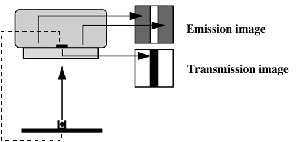
\includegraphics[width=\figone]{figs/fig_specttrans.pdf}
\caption{\label{fig:specttrans} \emph{Scanning transmission source in a gamma
camera. An electronic window is synchronized with the source, improving
separation of transmission and emission counts.}}
\end{figure}

The transmission isotope is selected to emit photons at an energy
different from the emission tracer. Thus, emission and transmission
photons can be separated, enabling simultaneous acquisition of
transmission and emission projections. In the scanning line source
configuration, an electronic window is moved in synchronization
with the source. Photons outside the electronic window cannot have
originated in the source, and must be due to scatter from emission
photons (if the energy of the emission isotope is
higher). Consequently, the electronic window improves the separation
already achieved with the energy windows.

Figure \ref{fig:pettrans} shows a typical PET transmission
configuration. One or a few rotating rod sources are used. In theory,
a single photon emitter could be used, since the position of the rod
sources is known at all times. However, current systems usually use a
positron emitter, so separation based on energy windowing is not
possible. Again, small electronic windows (selecting only projection
lines involving a detector close to the source) are used, which reduce
the emission contamination with a factor of about 40. The remaining
contamination can be estimated from an emission sinogram acquired
immediately before or after the transmission scan.

\begin{figure}[tb]
\centering
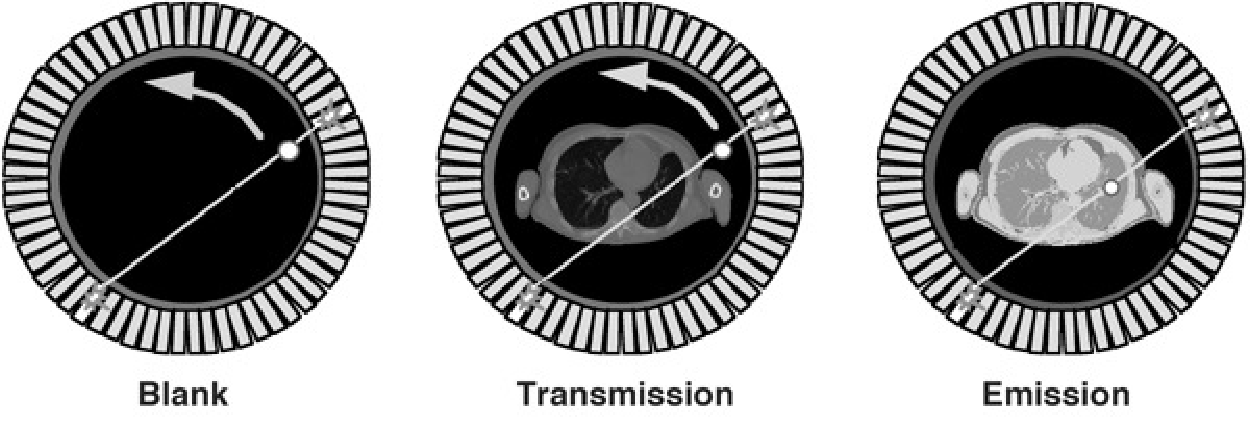
\includegraphics[width=\figbig]{figs/fig_pettrans.pdf}
\caption{\label{fig:pettrans} \emph{Rotating transmission source in PET. As a
reference, a blank scan is acquired daily.}}
\end{figure}

\begin{figure}[tb]
\centering
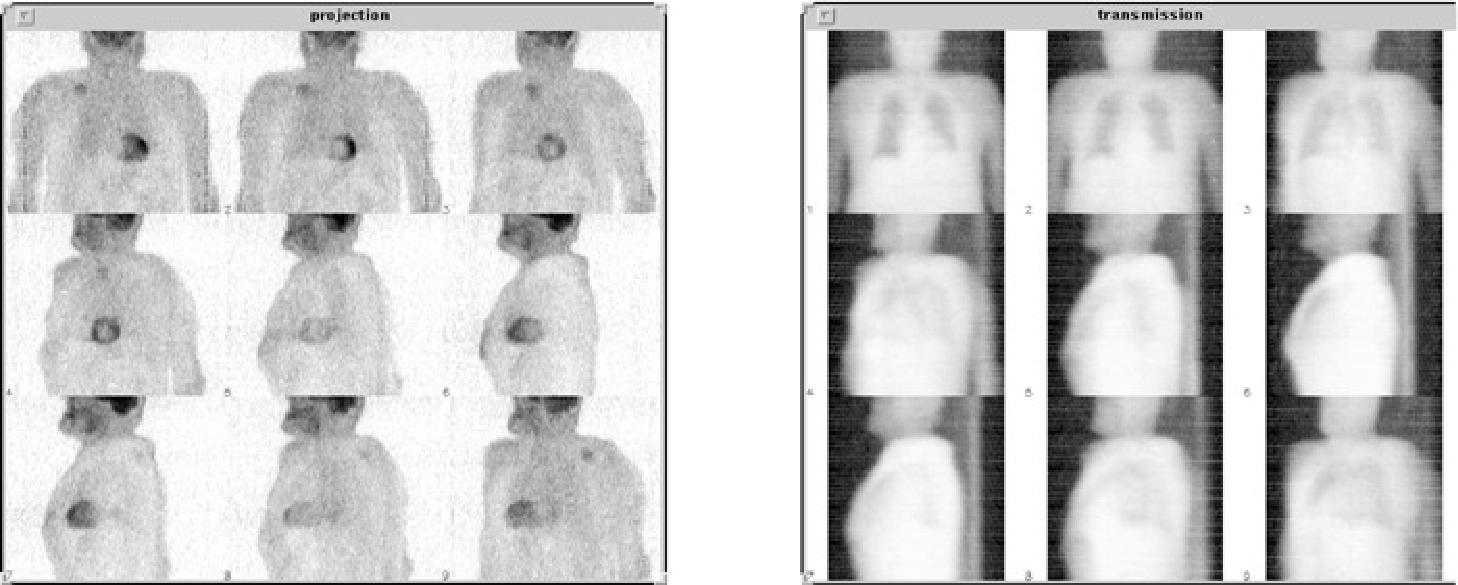
\includegraphics[width=\figbig]{figs/fig_transproj.pdf}
\caption{\label{fig:transproj} \emph{Left: emission PET projections. Right:
transmission projections of the same patient.}}
\end{figure}

For every projection line, we also need to know the number of photons
emitted by the source (see eq. (\ref{eq:attencor}) and
(\ref{eq:ct_proj2})). These values are measured during a blank
scan. The blank scan is identical to the transmission scan, except
that there is nothing in the field of view. Blank scans can be
acquired over night, so they do not increase the study duration. Long
acquisition times can be used, to reduce the noise in the blank scan.

\section{Transmission reconstruction}
%%%%%%%%%%%%%%%%%%%%%%%%%%%%%%%%%%%%%
For PET, only the ratio between blank and transmission is required. However,
it is useful to reconstruct the transmission image for two reasons. First,
although the image quality is very poor compared to CT, it provides some
anatomical reference which may be valuable to the physician. Second, the
attenuation along a projection line may be computed from the reconstructed
image. This improves the signal to noise ratio. Indeed, when computed from the
reconstruction, the entire blank and transmission sinogram contribute to the
estimated attenuation coefficient. In contrast, an estimate computed from the
ratio of blank and transmission scans is based on a single blank and
transmission pixel value.

For SPECT, the transmission measurement must be reconstructed, because the
reconstruction values are required to compute the coefficient $c_{ij}$ in
(\ref{eq:jnmlem}) or in other iterative algorithms.

All what has been said about reconstruction of emission scans can be done for
transmission scans as well. However, there is an important difference. In
emission tomography, the raw data are a weighted sum of the unknown
reconstruction values. In transmission tomography, the raw data are
proportional to the exponent of such a weighted sum. As a result of this
difference, the MLEM algorithm cannot be applied directly, so several new
ones have been presented in recent literature. Similarly as in the emission
case, one can use a non-trivial prior distribution for the reconstruction
images. In that case, the reconstruction is called a maximum-a-posteriori
algorithm or MAP-algorithm (see section \ref{sec:bayes}).

The prior $p(\Lambda)$ is the probability we assign to the image $\Lambda$,
independently of any measurement. To suppress the noise, the prior probability
function is designed such that it takes a higher value for smoother images.
This is typically done by computing the sum of all squared differences between
neighboring pixels, but many other functions have been invented as well.
Such functions have been successfully used, both for emission and transmission
tomography. In the case of transmission tomography, we also have prior knowledge
about the image values: the linear attenuation coefficient of human tissues is
known. Thus, it makes sense to design prior functions that return a higher value
when the pixel values are closer to the typical attenuation values encountered
in the human body.

Figure \ref{fig:pettranslang} shows the reconstructions of a 10 min
transmission scan. The same sinogram has been reconstructed with filtered
backprojection, ML and MAP. Because the scan time is fairly long, image
quality is reasonable for all algorithms.

Figure \ref{fig:pettranskort} shows the reconstructions of a 1 min
transmission scan obtained with the same three algorithms. In this short scan,
the noise is prominent. As a result, streak artifacts show up in the filtered
backprojection image. The ML-image produces non-correlated noise with high
amplitude. As argued in section \ref{sec:regularization}, this can be expected,
since the true number of photons attenuated during the experiment in every
pixel is subject to statistical noise. And if that number is small, the
relative noise amplitude is large. The MAP-reconstruction is much smoother,
because the prior assigns a low probability to noisy solutions. This image is
a compromise between what we know from the data and what we (believe to) know
a priori.

\begin{figure}[tb]
\centering
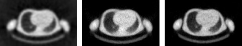
\includegraphics[width=\figbig]{figs/fig_pettranslang.pdf}
\caption{\label{fig:pettranslang} \emph{Reconstruction of a PET transmission
scan of {\bf 10 min}. Left: filtered backprojection; Center: MLTR; Right: MAP
(Maximum a posteriori reconstruction).}}
\end{figure}

\begin{figure}[tb]
\centering
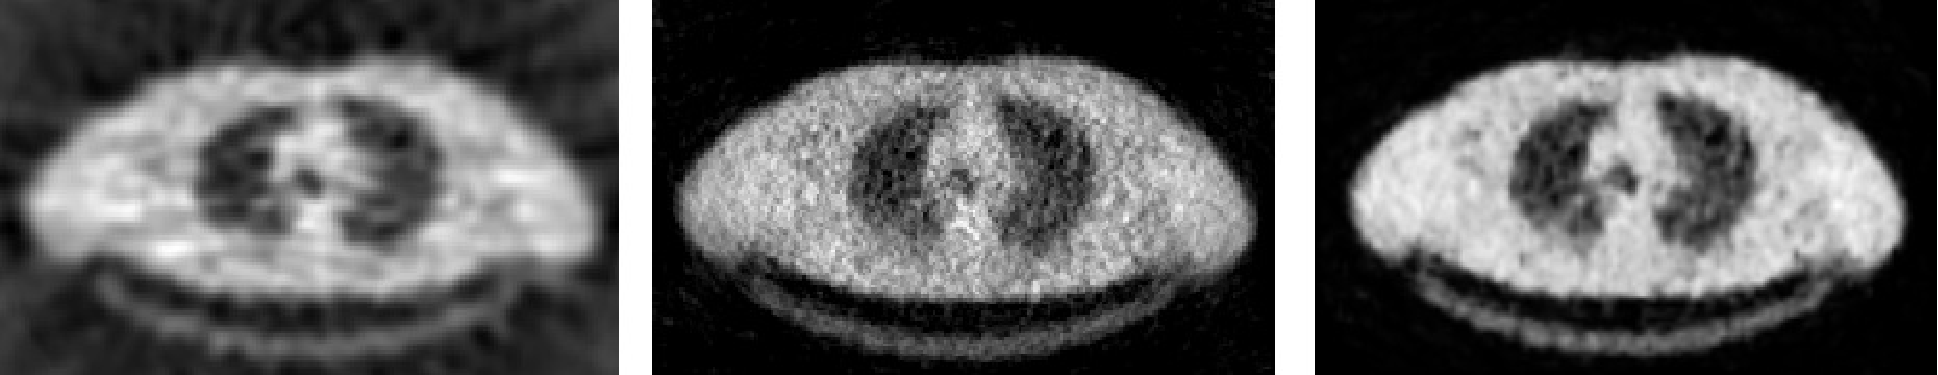
\includegraphics[width=\figbig]{figs/fig_pettranskort.pdf}
\caption{\label{fig:pettranskort} \emph{Reconstruction of a PET transmission
scan of {\bf 1 min}. Left: filtered backprojection; Center: MLTR; Right: MAP
(Maximum a posteriori reconstruction).}}
\end{figure}

Transmission scanning has never become very popular in SPECT, because
the physicians felt that their diagnosis was not adversely affected by
the attenuation-artifacts (i.e. artifacts caused by ignoring the
attenuation) and because it increases the cost of the gamma camera. In
PET, those artifacts tend to be more severe, and transmission scanning
has been provided and used in almost all commercial PET
systems. However, since the introduction of PET/CT, the CT image has
been used for attenuation correction, and most PET/CT systems do no
longer have the hardware for PET transmission scanning.

\section{Combined PET/CT}
%%%%%%%%%%%%%%%%%%%%%%%%%
\subsection{The CT system}
%=========================
\begin{figure}[tbp]
\centering 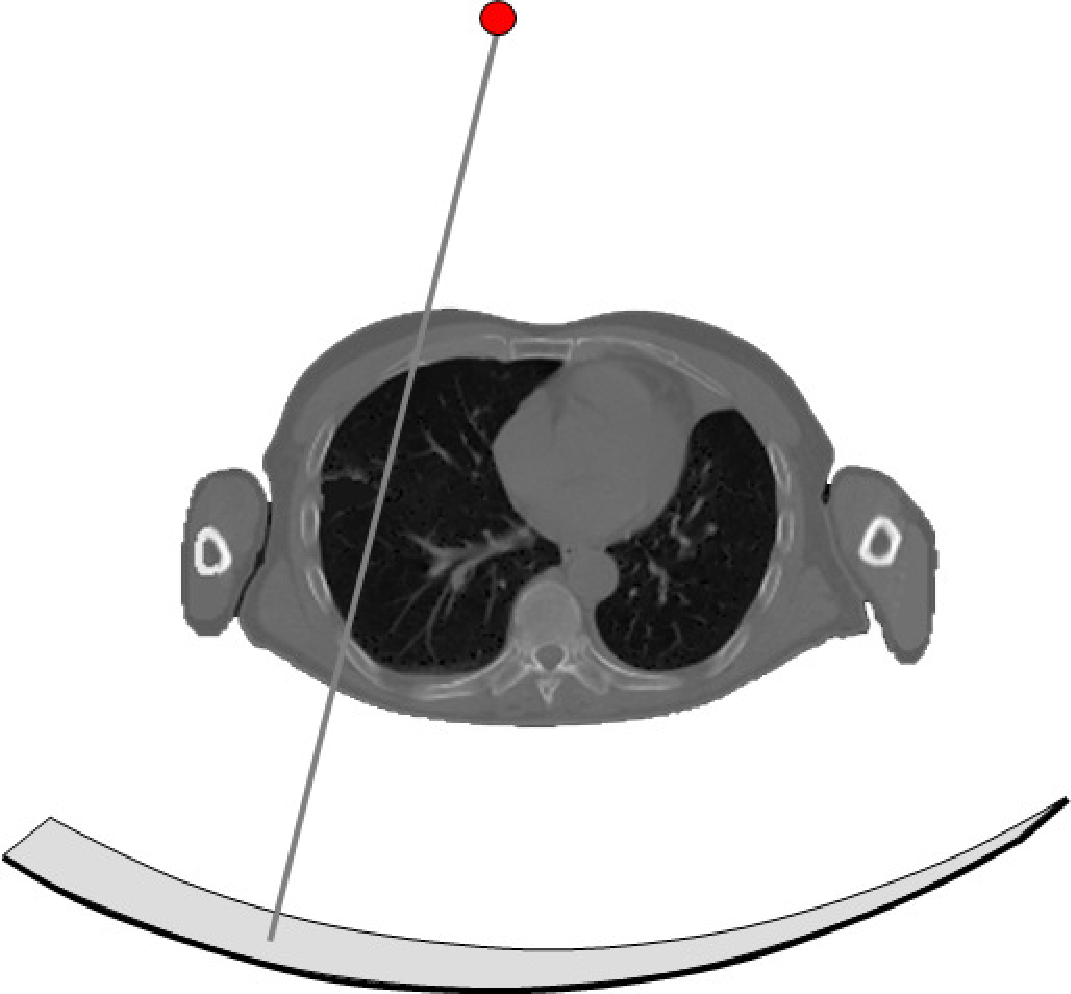
\includegraphics[width=0.6\figbig]{figs/fig_ct.pdf} 
\caption{\label{fig:ct} \emph{A CT system consists of a collimated
    X-ray tube and a detector mounted on a rotating gantry. The
    detector has tens to hundreds of rows, each consisting of about a
    thousand detector elements}}
\end{figure}
%
The principle of the CT system (fig. \ref{fig:ct}) is similar to that
of PET transmission scanning, but the implementation is far more
sophisticated and performant. For the transmission source, an X-ray
tube is used. A high voltage of $H$ kV (typically $H$ equals about
80-140 kV) frees electrons in the kathode and accelerates them, such
that they hit the anode with a kinetic energy of $H$ keV per electron.
That energy is converted mostly to heat, but also to X-rays
(bremsstrahlung and characteristic X-rays). The X-ray tube is
collimated, such that all the radiation is absorped except if it is
propagating towards the detector.

The detector surface is cylindrical, with the X-ray tube located on
the axis of the cylinder. In the axial direction it is several cm
long, the transaxial size is about a meter to ensure minimal
trunctation when imaging the human body. The detector consists of a
matrix of detector elements, organized in tens up to hundreds of rows,
each containing up to a thousend detector elements. Current CT-systems
use integrating detectors: they measure the total energy incident on
the detector during a small time interval.

During the calibration, blank scans (aka air scans) are acquired at
different energies. As already explained above, a blank scan and
transmission scan (acquired at the same energy) are combined to
compute the total attenuation along a particular line:
\begin{equation}
  \ln\left(\frac{\mbox{blank}(i)}{\mbox{transmission}(i)}\right) 
     = \int_s^d \mu(x) dx, \label{eq:totatten}
\end{equation}
where $s$ and $d$ are the position of the source and the detector on
the projection line corresponding to detector element $i$.

When the line integrals (\ref{eq:totatten}) are available, the
attenuation image $\mu$ can be reconstructed, either analytically
(with a filtered backprojection algorithm) or iteratively (e.g. with a
maximum likelihood algorithm). The pixel values of the reconstructed
image would then represent (approximately) the attenuation of the
tissues at the average energy of the X-ray photons (typically around
70 keV). To make the image independent of the chosen energy of the
X-ray tube, the image values are converted to so-called Hounsfield
units (HU) as follows:
\begin{equation}
  \mbox{HU-value(x,y,z)} 
    = 1000 \frac{\mu(x,y,z) - \mu_{\mbox{water}}}{\mu_{\mbox{water}}},
\end{equation}
where $(x,y,z)$ represents the coordinate of the considered voxel in
the CT image.  Consequently, the attenuation of vacuum corresponds to
-1000 HU, and the attenuation of water to 0 HU.

\subsection{The PET/CT system}
%=============================
In oncology, patients often undergo a CT and a PET $^{18}$F-FDG scan. The
CT-image provides very fine anatomical detail, but cannot easily differentiate
malign tumors from necrotic or benign tissue. The PET-image shows regions with
increased metabolic activity, but provides limited anatomical detail.
Obviously, the physicians would like both at the same time.

Around 2000, the first PET/CT prototype system has been introduced. A
PET-camera and a CT-scanner are combined in a single gantry and share
the same patient bed (fig \ref{fig:petct}). By scanning phantoms
visible in both systems (e.g. radioactive point or rod sources) the
geometrical aligment between both systems is determined. That ensures
that for each CT-voxel the corresponding PET-voxel can be found.
%
\begin{figure}[tbp]
\centering
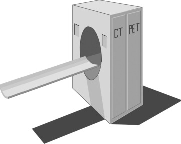
\includegraphics[width=0.6\figbig]{figs/fig_petct.pdf}
\caption{\label{fig:petct} \emph{A PET/CT system consists of a PET and
 a CT system, sharing the same patient table.}}
\end{figure}

Typically, a patient examination starts with a helical CT-scan from the
head to the pelvis, which is completed in about 15 seconds. Then the
PET-scan is acquired: this involves about 7 acquisitions at subsequent
bed positions, where each acquisition provides an image volume
extending over 10 to 15 cm. At 2 to 4 minutes per bed position this
requires about 15 to 30 min, so the whole examination would require
about 20 to 35 min. Assuming that the patient does not move during the
entire procedure, the two images are perfectly aligned, and the
physicians can see the the function and anatomy at the same time, as
illustrated in fig \ref{fig:petctimg}.
%
\begin{figure}[tb]
\centering
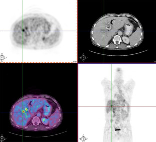
\includegraphics[width=0.7\figbig]{figs/fig_petctimg.pdf}
\caption{\label{fig:petctimg} \emph{Images from a PET/CT system, allowing
simultaneous inspection of anatomy and function.}}
\end{figure}

It has been shown that this combined imaging improves the diagnostic
procedure considerably, in particular in oncology, and the PET/CT
system has been accepted with great enthousiasm. All PET-manufacturers
offer PET/CT systems, and since 2006 it has even become virtually
impossible to buy a PET-system without CT. Also SPECT-CT systems are
being offered now, although they are not nearly as successful (yet?)
as the PET/CT systems.

\subsection{CT-based attenuation correction}
%===========================================
In the beginning, the PET in the PET/CT system still had a transmission
source, allowing a comparison between the PET-transmission image (using a
positron emitter for transmission source) and the CT-image. However,
PET-transmission scanning is slow and current systems use the CT-image for the
PET attenuation correction.

An obvious advantage of the CT image is that it is nearly noise-free:
there are millions of photons per detector element, whereas a
PET-transmission scan typically has a few hundered per detector. But
there are problems too. The two most important problems are the
conversion of the linear attenuation coefficients and dealing with
patient motion.

\subsubsection{Conversion of the attenuation coefficients}
%---------------------------------------------------------
The attenuation of photons in CT and PET is dominated by the photo-electric and
Compton interactions. The photo-electric effect varies approximately with
$(Z/E)^3$, while the Compton effect hardly varies with photon energy $E$ and
atomic number $Z$. The photons produced by positron-electron annihilation have
an energy of 511 keV. However, the radiation used in a CT-scanner is very
different, so we will have to convert the CT-attenuation values from the CT
energy to 511 keV, if we want to use them for PET attenuation coefficients.

The CT produces radiation by bombarding an anode with electrons in a vacuum
tube. The electrons are accelerated with an electric field, which can usually
be adjusted in a range of about 80 to 140 kV, so they acquire a kinetic energy
of 80 to 140 keV. They hit the anode where they are stopped. Part of their
energy is dissipated as Bremsstrahlung, which produces a continuous spectrum.
In addition, the electrons may also knock anode electrons out of their shell
(e.g. the K-shell). A higher shell electron (e.g. from the L-shell) will then
move to the vacant lower energy state, producing a characteristic radiation of
$E_L - E_K$. So if the CT voltage is set to 140 kV, the CT-tube produces
radiation with a spectrum between 0 and 140 keV (fig \ref{fig:ctspectrum}).
%
\begin{figure}[tbp]
\centering
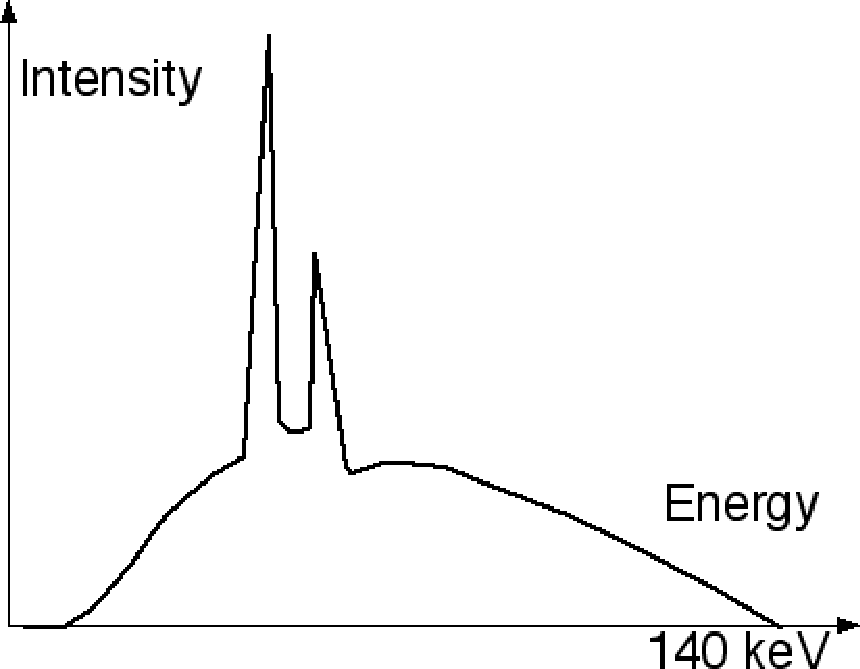
\includegraphics[width=0.5\figbig]{figs/fig_ctspectrum.pdf}
\caption{\label{fig:ctspectrum} \emph{Typical CT spectrum with continuous
Bremsstrahlung and a few characteristic radiation peaks.}}
\end{figure}

Human tissue consists mostly of very light atoms. For attenuation
correction, these tissues can be well approximated as mixtures of air
or vacuum (no attenuation) and water. The attenuation of water is
about 0.096/cm at 511 keV, and about 0.19 at 70 keV, which is the
"effective" energy of the CT-spectrum. Assuming that everything in the
human body is a mixture of water and vacuum, we only need a single
scale factor equal to 0.096 / 0.19. But of course, there is also bone.
One can apply the same trick with good approximation: we regard
everything denser than water as a mixture between water and
bone. Dense bone has an attenuation of about 0.17/cm at 511 keV, and
about 0.44/cm at 70 keV. This yields the piecewise linear conversion
function shown in fig \ref{fig:petctconversion}.
%
\begin{figure}[tbp]
\centering
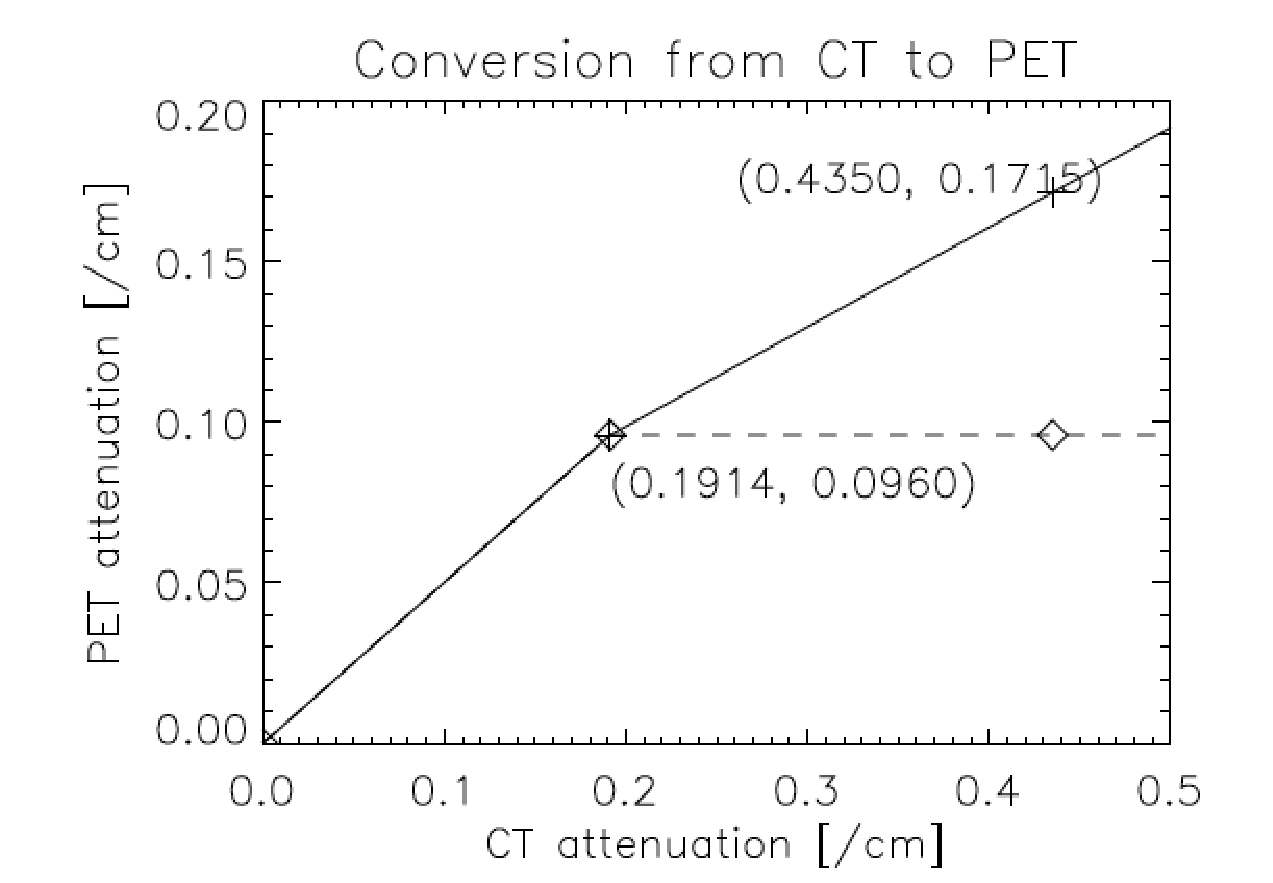
\includegraphics[width=0.6\figbig]{figs/fig_petctconversion.pdf}
\caption{\label{fig:petctconversion} \emph{Piecewise linear conversion
typically used in PET/CT software to move attenuation coefficients
from 70 to 511 keV.}}
\end{figure}

\begin{figure}[tbp]
\centering
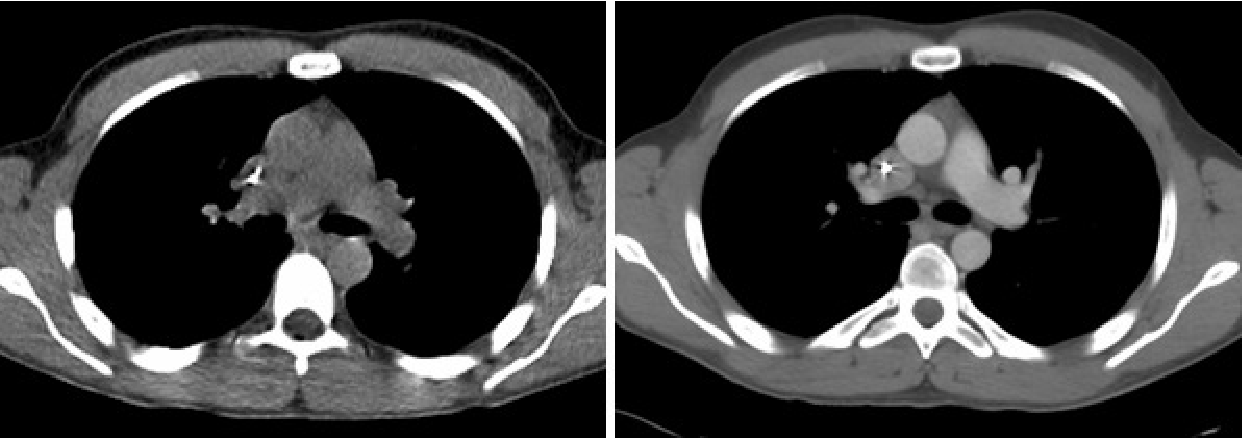
\includegraphics[width=0.9\figbig]{figs/fig_CTcontrast.pdf}
\caption{\label{fig:CTcontrast} \emph{Left: CT image, acquisition with
    30 mAs and no contrast. Right: CT image, acquisition with 140 mAs
    and intravenously injected contrast agent.}}
\end{figure}

This scaling works reasonably well, except if a contrast agent is used
during a diagnostic CT-scan. Contrast agents are used to improve the
diagnostic value of the CT-image. Often a contrast agent is injected
intravenously to obtain a better outline of well perfused
regions. This is illustrated in fig \ref{fig:CTcontrast}, which
compares a CT image acquired with lower radiation dose and no
contrast, to an image obtained with a higher radiation and intravenous
contrast. Other contrast agents have to be taken orally, and are used
to obtain a better visualization of the digestive tract. These
contrast agents usually contain iodine, which has very high
attenuation near 70 keV due to photo-electric effect (which is why
they are effective for CT-imaging), but the attenuation is hardly
higher than that of water at 511 keV (mostly Compton interactions). As
a result, the piecewise conversion produces an overestimation of the
PET-attenuation in regions with significant contrast uptake. This
matter is currently being investigated, no standard solution exists.

A related problem is that of metal artifacts. Because the attenuation
of metal prostheses or dental fillings is extremely high at 70 keV,
such objects can attenuate almost all photons. The number of acquired
photons is in the denominator of equation (\ref{eq:attencor}), so the
CT-reconstruction gets into problems when the number of acquired
photons goes to zero. This numerical instability can produce artifacts
in the CT-reconstruction, which will propagate into the PET image via
the CT-based attenuation correction. (Partial) solutions exist, but
currently, they are not yet included in commercial CT-software.

\subsubsection{Geometrical calibration}
%--------------------------------------
To make sure that the PET and CT images are well aligned
(fig. \ref{fig:petctimg}), careful geometrical calibration of the two
systems is mandatory. This is done by acquiring a phantom which is
clearly visible in both modalities. E.g., one of the vendors (Siemens)
uses a phantom consisting of two non-coplanar rod sources. These rods
are a made of stainless steel, have a diameter of about a mm and are
filled with $^{68}$Ge. These rods are clearly visible in both PET and
CT, and it is relatively easy to compute the transformation (6 degrees
of freedom) required to accurately align the images. The same
transformation is then applied to align the patient images. This
transformation usually remains valid until something changes, which is
typically the case when something must be repaired (X-ray tube
replacement, PET detector replacement etc.). For such actions, the two
systems are pulled apart. After combining them again, the spatial
alignment could be change by a few mm, so a new calibration is then
required.

\subsubsection{Patient motion}
%-----------------------------
The time between the helical CT-scan and the last PET-scan is about half an
hour. That is a long time to ly motionless, and in most PET/CT images one can
see small positional mismatches due to patient motion. A similar mismatch is
caused by breathing. The CT-scan is very fast compared to the breathing cycle,
and essentially takes an image at one point of that cycle. In contrast, the
PET-scan runs for a few minutes per bed position, and produces an image
averaged over the breathing cycle. This causes motion blur in the PET image,
and a registration mismatch with the corresponding CT image. The mismatch may
yield attenuation correction artifacts in the PET image. An example of such an
artifact is shown in figure \ref{fig:petctbreathing}. The CT has been taken at
maximum inhalation, causing the lungs in the CT-image to be larger than in the
PET image. The patient increased his lung size mostly by a displacement of the
diaphragm. The CT-based attenuation correction underestimates the attenuation
at the dome of the liver (because the computer thinks this part has undergone
lung attenuation, and the lungs are far less dense than the liver). This
undercorrection, then, yields a decrease of apparent tracer uptake, making the
activity in this part of the liver similar to that in the lung. As a result,
the liver tumor seems to show up in the lung. The figure also shows an image
obtained with attenuation correction based on a (well matched) transmission
scan with a positron emitter, clearly showing that the tumor is in the
liver.

Another example is given in figure \ref{fig:petctatcor}. Because of
potential attenuation correction artifacts, it is good practice to
always make a reconstruction of the PET image without attenuation
correction (fig \ref{fig:petctatcor}.A). This image has of course
always many artifacts too, but these artifacts tend to be similar in all
patients, so one can learn to read such images. Comparison of the
image with and without attenuation correction may reveal subtle
attenuation correction artifacts, which otherwise might lead to the
wrong diagnosis. Such an artifact is present in the brain in fig
\ref{fig:petctatcor}.C, which shows a left-right asymmetry caused by a
motion artifact.

%
\begin{figure}[tbp]
\centering
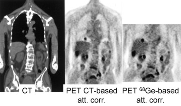
\includegraphics[width=0.7\figbig]{figs/fig_petctbreathing.pdf}
\caption{\label{fig:petctbreathing} \emph{PET/CT attenuation artifact
due to breathing. The tumor is really located in the liver, but the
mismatch with the CT and the resulting attenuation correction errors
make it show up in the lung.This figure is from a paper by Sarikaya,
Yeung, Erdi and Larson, Clinical Nuclear Medicine, 2003; 11: 943}}
\end{figure}

\begin{figure}[tbp]
\centering
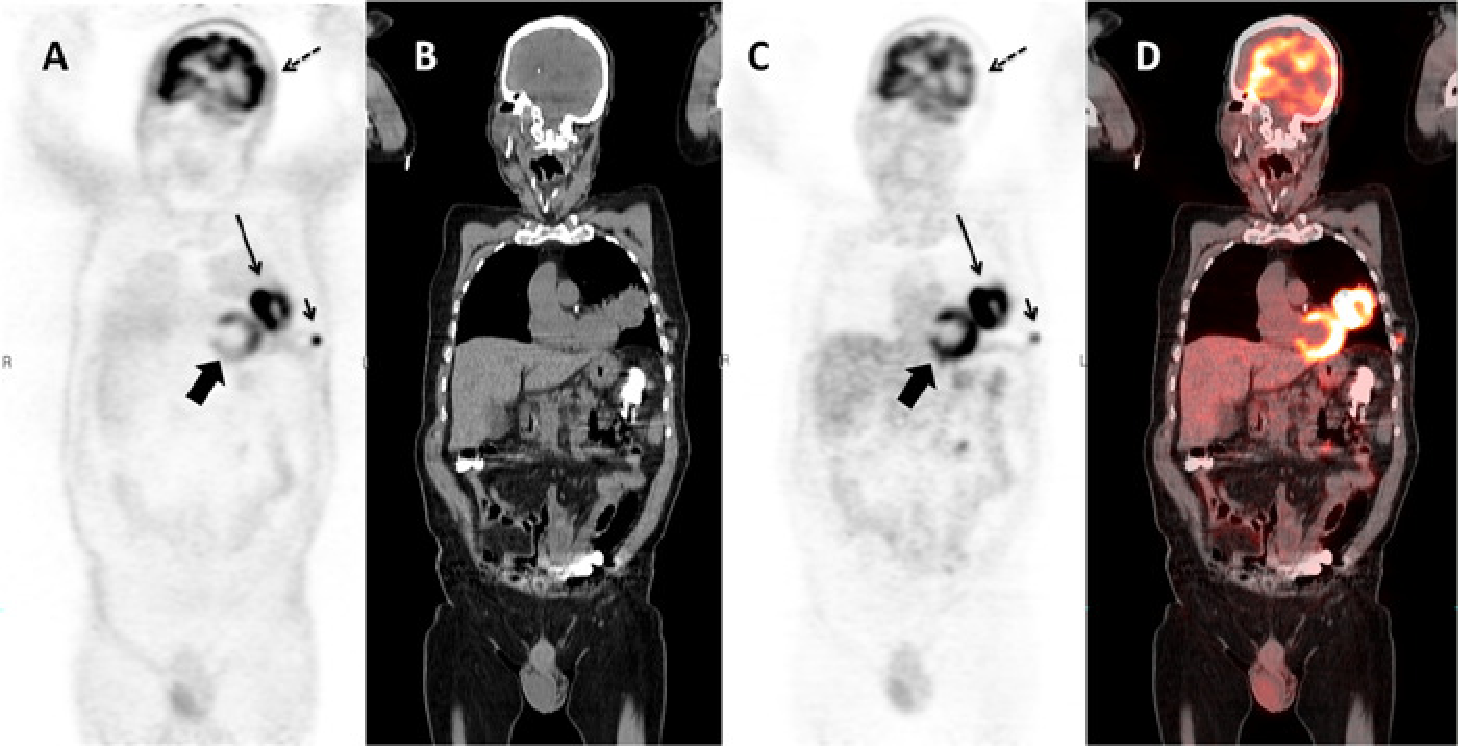
\includegraphics[width=0.9\figbig]{figs/fig_petctatcor.pdf}
\caption{\label{fig:petctatcor} \emph{Coronal slice of a whole body
PET/CT study reconstructed without (A) and with (C) attenuation
correction based on a whole body CT (B). PET and CT are combined in a
fusion image (D). The relative intensity of the subcutaneous
metastasis (small arrow) compared to the primary tumor (large arrow)
is much higher in the non corrected image than in the corrected one,
because the activity in this peripheral lesion is much less attenuated
than the activity in the primary tumor. A striking artifact in (A) is
the apparent high uptake in the skin and the lungs. Note also that
regions of homogenous uptake, such as the heart (thick arrow), are no
longer homogenous, but show a gradient. The uptake in the left side of
the brain (dotted arrow) is apparently lower than in the contralateral
one in (C). The fusion image shows that the head did move between the
acquisition of the CT and the emission data, resulting in an apparent
decrease in activity in the left side of the brain due errors in the
attenuation correction.}}
\end{figure}

The correction of these artifacts is a current research topics, no standard
solutions exist.